\documentclass[../main.tex]{subfiles}
\begin{document}
\section{\label{sect:NRQFT}Applications in nonrelativistic matter: ultracold atomic gases}
%
\begin{figure}[t]
  \centering
  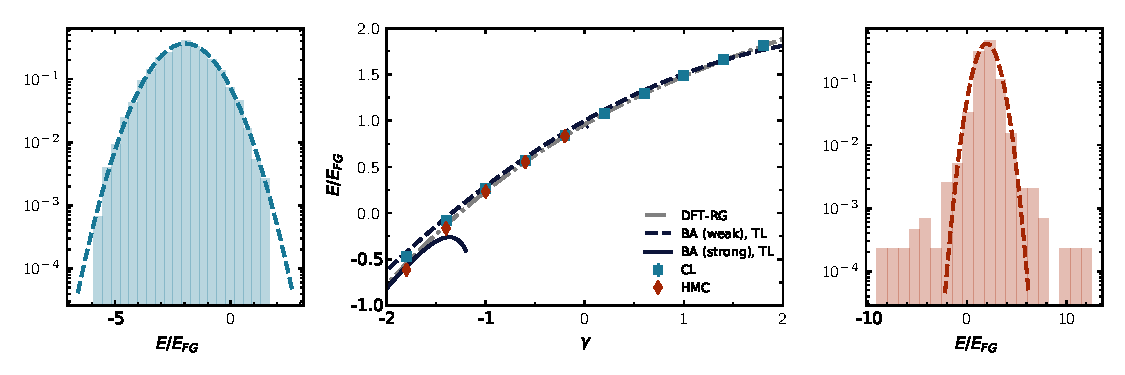
\includegraphics[width=\columnwidth]{./5applications-NREL/1d_bal_eos.pdf}
  \caption{\label{fig:1d_bal_eos}  (Left) Log-histogram for sampled ground-state energies at strong attractive coupling $\gamma = -3.0$. Perfect gaussian behavior is observed (dashed line). (Center) Ground-state energy of $N = 5 + 5$ fermions as a function of the dimensionless coupling $\gamma$. The CL results (blue squares) are compared to HMC results (red diamonds) as well as to the Bethe-Ansatz solutions for strong and weak coupling (solid and dashed lines, respectively) and results obtained by a DFT-RG approach \cite{0954-3899-44-1-015101} (dashed-dotted line). (Right) Log-histogram for sampled ground-state energies at strong repulsive coupling $\gamma = 3.0$. Heavy tails of the distributions (as compared to a Gaussian, dashed line) spoil the correctness criterion.}
\end{figure}
%

In contrast to the relativistic case, applications of CL to nonrelativistic matter remain largely in their infancy
(notwithstanding notable work such as Ref.~\cite{PRC2001026303}).
As described below, there have been attempts to characterize bosons as well as fermions in a variety of situations,
but as of this writing only one calculation has been successfully carried out for a strongly coupled fermionic system in 3D at finite temperature.
Nonrelativistic systems have difficulties of their own in the form of phase transitions and strongly coupled regimes, but they do not feature quintessential
(and technically challenging) QCD elements such as non-abelian gauge fields. Nevertheless, as we shall see, some of the challenges faced by CL calculations are
universal, as are the ideas to tackle them and the tools to diagnose them (see \secref{formalism}).

Among the vast array of nonrelativistic systems that remain to be explored, some pressing candidates remain across different areas,
such as the repulsive 2D Hubbard model, the polarized electron gas, spin-isospin polarized nuclei, and neutron and nuclear matter, to name a few.
We hope that the growing applications outlined in this section will lead to further work in those areas.

%%%%%%%%
\subsection{Nonrelativistic bosons}

One of the pioneering applications of CL to nonrelativistic systems in the modern era (roughly within the last decade) concerned the study of a bosonic quantum
field theory in a rotating frame~\cite{PhysRevA92043628}.
The number density and condensate fraction with no rotation computed via CL was found to agree with mean-field calculations, and when rotation
was introduced, the CL results showed quantized circulation for high condensate fraction. This is consistent with vortex formation in rotating
superfluids, a phenomenon which has been directly observed using rotating ultracold bosonic atoms. The results for the circulation
using CL do not agree with mean-field calculations for small condensate fraction, as expected due to the breakdown of mean-field
theory to describe a system with strong quantum fluctuations. Aside from this brief exploration, the application of CL to
circumvent the sign problem in systems of nonrelativistic systems, in particular bosons, remained scarce.
%In this section we elaborate on more recent CL studies of nonrelativistic fermions in a variety of situations that display a sign problem,
%including cases, such as certain 1D systems, where the sign problem can be avoided by other methods but which can be used as test cases for CL.

%%%%%%%%
\subsection{Nonrelativistic fermions in one dimension}
%Recently, advances have been made in applying CL to fermionic systems that suffer from a sign problem. The ground state energy of mass-imbalanced fermions was computed via CL and showed agreement with other methods. Furthermore, the results obtained by CL demonstrated better-controlled statistical uncertainties and results were obtained beyond the regimes accessible by other methods~\cite{PRD96094506}. Some instability was observed in this system for repulsive interactions, particularly as the repulsive coupling grows in size, likely due to zeroes in the fermion determinant~\cite{2017arXiv171011421R}.
%expand on these

%Recent work on one-dimensional fermionic systems calculated the density and pressure equations of state, computed virial coefficients using the particle projection method, and compared Langevin results with third-order lattice perturbation theory results ~\cite{PRD95094502}. In one dimension, lattice perturbation theory is able to circumvent the sign problem, so the close agreement of the CL results with perturbation theory in one dimension confirms the viability of CL to fermionic systems suffering from a sign problem. The pressure, density, and magnetization of spin-polarized fermions has also been computed using CL, and the results are consistent with N$3$LO perturbation theory in $1$D~\cite{LatticeProceedingsALoheac2017}. %We should update this citation to the paper once it's published

%---

One-dimensional (1D) Fermi gases have drawn considerable interest in the past, when exact solutions for various models have been derived by the use of the so-called Bethe ansatz (see e.g., Ref.~\cite{RevModPhys.85.1633} for an extensive review). The availability of these exact solutions, paired with a relatively modest computational cost, make these systems excellent benchmark scenarios for any newly devised method, such as the CL approach for nonrelativistic quantum matter.  Moreover, 1D systems have become accessible in experiments in recent years, which provides yet another motivation to study these exotic and intrinsically strongly interacting systems.
%
\begin{figure}[t]
  \centering
  \begin{subfigure}[t]{0.56\columnwidth}
    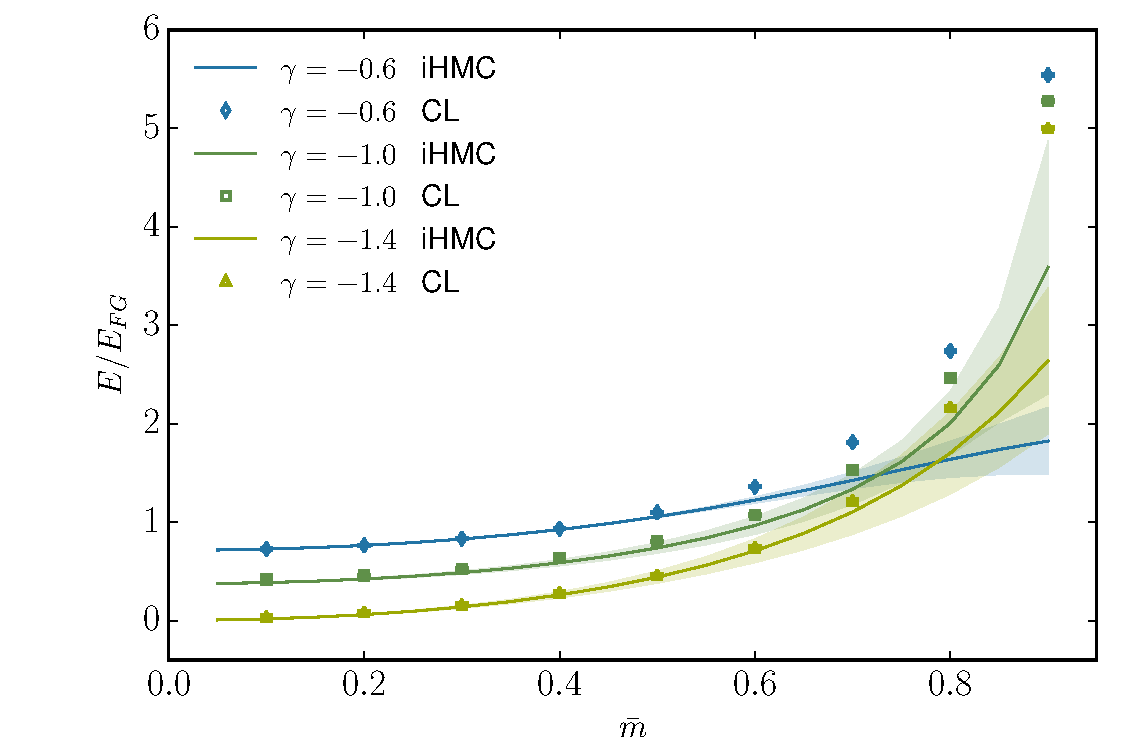
\includegraphics[width=\columnwidth]{./5applications-NREL/1d_ihmc_cl.pdf}
  \end{subfigure}
  \begin{subfigure}[t]{0.4\columnwidth}
    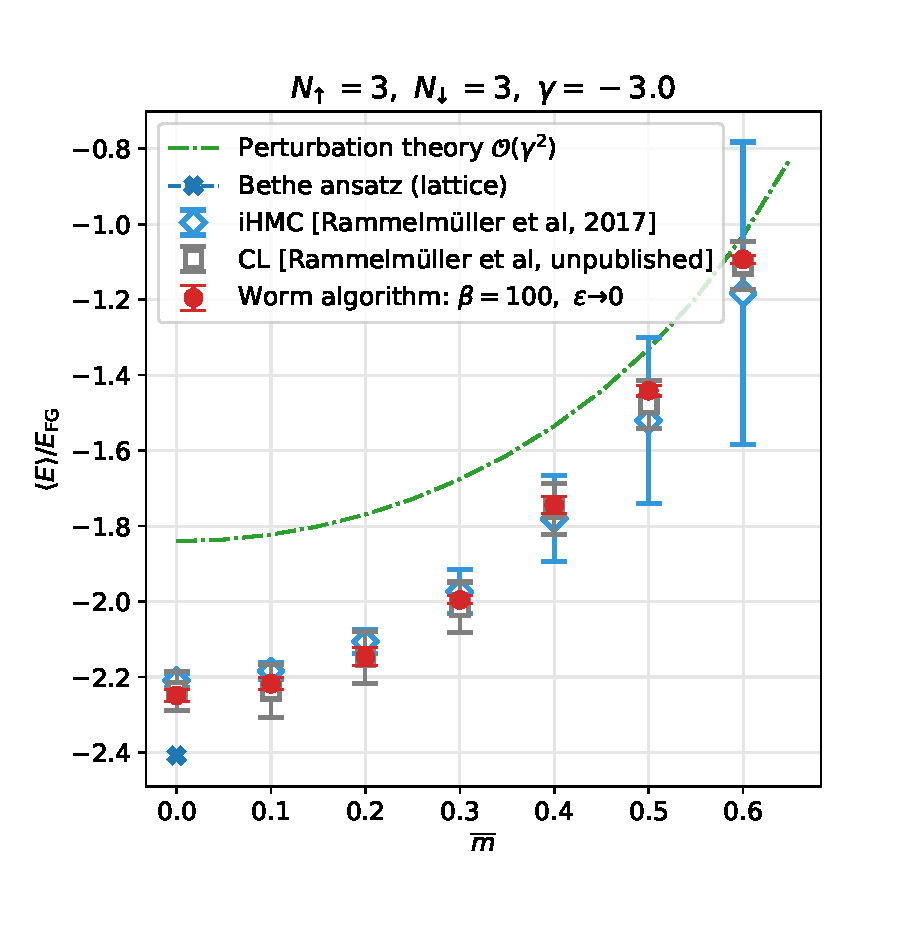
\includegraphics[width=\columnwidth]{./5applications-NREL/1d_duke_compare.pdf}
  \end{subfigure}
  \caption{\label{fig:1d_mib_eos} (Left) Comparison of iHMC and CL as a function of relative mass-imbalance $\bar m$ for $N_\uparrow+N_\downarrow = 5+5$ particles at fixed interaction streghts $\gamma$. (Right) Ground-state energy of $N = 3 + 3$ fermions as a function of $\bar m$ as obtained with the Worm algorithm \cite{PhysRevD.99.074511} in comparison with CL results as well as iHMC values and perturbation theory. The plot is taken from Ref.~\cite{PhysRevD.99.074511}.}
\end{figure}
%

It is worthwhile to note here that in the special case of 1D it is often possible to re-write relativistic and nonrelativistic models using dual variables, in a way that avoids sign problem. One would be able to compute quantities by conventional Monte Carlo methods. While this is an option in 1D, those approaches do not generalize to higher dimensions, in contrast to the CL method. In fact, the dimensionality of the problem is mainly a question of computational effort and all insights gained on the numerical behavior of CL simulations carry over to higher dimensions.

In this section, we will review recent advances that have been made in applying CL to one-dimensional fermionic systems that suffer from a sign problem. Specifically, we will discuss systems at zero temperature featuring attractive and repulsive interactions, finite spin-polarization as well as asymmetry in the masses of the fermions in \secref{fermions_gs_1d}. Furthermore, we recall results obtained at finite temperature in \secref{fermions_ft_1d} where repulsively interacting fermions are shown as well as systems at asymmetric chemical potential.

%%%%%%%%%%%%%%%%%%%%%
\subsubsection{1D fermions in the ground state \label{sect:fermions_gs_1d}}
In the following, we will consider a systems of $N = N_\uparrow + N_\downarrow$ fermions at fixed linear lattices of $N_x$ sites, which corresponds to working in the canonical ensemble. The physics in 1D is set by the dimensionless interaction parameter $\gamma = g/n$ where $g$ is the bare interaction and $n$ is the linear particle density.

\paragraph{Balanced systems}
%
As a first benchmark of the CL method in the ground state, the spin- and mass-balanced Fermi gas was investigated in Ref.~\cite{PRD96094506}. A comparison to various other methods is shown in \figref{1d_bal_eos}, where generally good agreement is apparent across the entire range of interactions shown. While the CL results shown are at $N = 5+5$ particles and a finite lattice of $N_x = 40$, the curves for the Bethe ansatz expansions (strong~\cite{1742-5468-2007-06-P06011} and weak~\cite{doi:10.1063/1.4964252} coupling) correspond to the thermodynamic limit (TL) of taking particle number and volume to infinity at constant density.
The agreement on the repulsive sides indicates sufficiently large box sizes. On the attractive side agreement is observed, however, larger spatial lattices are needed as is suggested by the slight discrepancy between CL and the volume-extrapolated HMC values of Ref.~\cite{PhysRevA.96.033635}, as well as results obtained by a DFT-RG approach in Ref.~\cite{0954-3899-44-1-015101}. Another possible source of systematic bias is the finite (adaptive) integration step of $\Delta t = 0.01$, which was used throughout this study. Although the $\Delta t$ dependence was checked in Ref.~\cite{PRD96094506}, where it was found that $\Delta t$ was sufficiently small (within the statistical uncertainty), the influence of $\Delta t$ could vary in other areas of parameter space, in particular with varying coupling strength.
%
\begin{figure}[t]
  \centering
  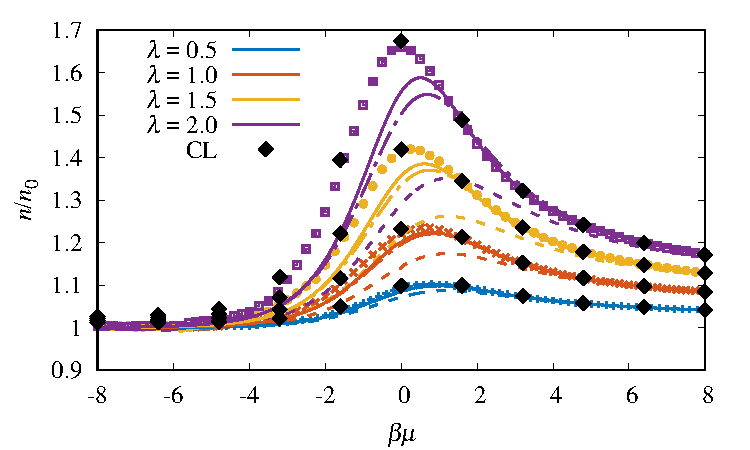
\includegraphics[width=0.49\columnwidth]{./5applications-NREL/PerturbationTheoryDensity.pdf}
  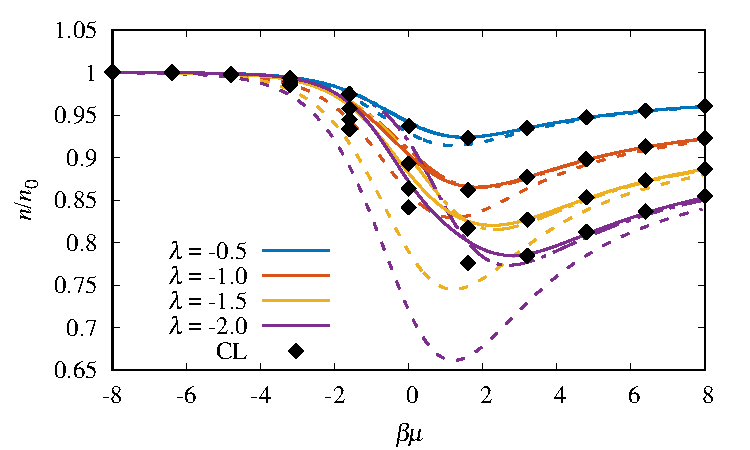
\includegraphics[width=0.49\columnwidth]{./5applications-NREL/PerturbationTheoryRepulsiveDensity.pdf}
  \caption{\label{fig:DensityEoSCL1DFiniteT} Density $n$ of the attractive (left) and repulsive (right) unpolarized Fermi gas in units of the density of the
	noninteracting system $n_0$, as shown for the dimensionless interaction strengths $\lambda = 0.5$, 1.0, 1.5, 2.0 (attractive), and $\lambda = -0.5$, -1.0, -1.5, -2.0
	(repulsive). The NLO (dashed line), N2LO (dash-dotted line), and N3LO (solid line) results of perturbation theory are displayed for each coupling and are
	compared with HMC results (see Ref.~\cite{PhysRevA.91.033618}) in the attractive case. For both plots, the black diamonds show CL results
	(RL for the attractive case), regulated with $\xi=0.1$ as described in the main text. Results were computed on a spatial lattice of $N_x = 80$ for CL and HMC, and of $N_x = 100$
  for perturbation theory. The statistical uncertainty of the CL results is estimated to be on
	the order of the size of the symbols, or less, as supported by the smoothness of those results.}
\end{figure}
%

While the agreement among the methods looks excellent, a closer look reveals interesting technical subtleties. During stochastic calculations it is instrumental to study histograms of all measured quantities to ensure correct behavior. As can be appreciated in the outer panels of \figref{1d_bal_eos}, two distinct behaviors were observed in different regimes: the strongly attractive case ($\gamma = -3.0$) displays well behaved, localized distributions; the strongly repulsive case ($\gamma=3.0$), on the other hand, exhibits a large amount of outliers with respect to an assumed Gaussian. The existence of so-called ``fat tails" renders the simulation problematic as this violates the conditions for correct behavior and thus undermines the validity of the CL approach. Therefore, it was conjectured that the CL values are possibly faulty in this parameter regime, which was later confirmed by a different few-body method \cite{PhysRevD.99.074511} based on dual variables and the worm algorithm. A more precise understanding of the behavior at strong repulsive interaction, and eventually its resolution, would be very useful.

\paragraph{Mass-imbalanced Fermi-Fermi mixtures}
{Mixtures of different fermion species, i.e. where the constituents have unequal masses, are challenging to address theoretically. While many 1D models are integrable via the Bethe ansatz, there is no such solution in the mass-imbalanced case. Nevertheless, these systems are of great interest as there are a number of experimental realizations available for these mixtures. The CL method can be straightforwardly extended to cover fermion systems with unequal masses by the use of spin dependent dispersion relations, i.e. a spin-dependent mass $m_\sigma$. To quantify the mass asymmetry between two species, the dimensionless relative mass-imbalance is introduced
%
\beq
  \bar m = \frac{m_\uparrow-m_\downarrow}{m_\uparrow+m_\downarrow},
\eeq
%
which is restricted to the interval $[0,1]$. While the use of spin-dependent dispersion relations is unproblematic from a conceptual viewpoint, there might arise numerical difficulties due to a separation of scales. Thus, one may use different parameterizations of the mass imbalance depending on the specific implementation of the algorithm.
}

In Ref.~\cite{PRD96094506} the mass-imbalanced few-body problem was studied and the average mass was fixed to $m_0 = 1$. In this way, a comparison is made possible to results obtained with the iHMC method (imaginary asymmetry -- introduced in \secref{ImaginaryAsymmetry}). A comparison is shown in the left panel of \figref{1d_mib_eos} for fixed values of the interaction strength $\gamma$. Excellent agreement of CL and iHMC is reported across a wide range of mass imbalances. Starting at $\bar{m} \sim 0.6$ the iHMC results start to deviate as a consequence of the instability of the analytic continuation. The CL results, on the other hand, remain smooth and precise up to high mass imbalances. The agreement between these different methods provides confidence that the CL method is suitable to study this problem.
Recently, a worldline algorithm was adapted to study mass-imbalanced few-body systems without a sign-problem \cite{PhysRevD.99.074511, Singh:2018pci} in 1D and its results have been compared to the CL values obtained in \cite{PRD96094506} (shown in the right panel of \figref{1d_mib_eos}). On the attractive side, excellent agreement is observed for all mass imbalances, which further validates the CL method in this setting. A comparison on the repulsive side, however, revealed that the CL values deviate from the wordline results, which is connected to the occurrence of heavy tails mentioned above and in Ref.~\cite{PRD96094506}. It remains to be shown whether mass-imbalanced Fermi mixtures with repulsive interactions in the ground state are accessible with CL.
%
\begin{figure}[t]
\floatbox[{\capbeside\thisfloatsetup{capbesideposition={right,top},capbesidewidth=0.4\textwidth}}]{figure}[\FBwidth]
{\caption{\label{fig:XiComparison}The normalized density $n/n_0$, where $n_0$ is the noninteracting result,
	for $\lambda=-1.0$ and $\beta\mu = 1.6$, as a function of the Langevin time $t$ for
	several values for the regulating parameter $\xi$ [see \equref{CLModifiedEqs}]. The result was computed on a spatial lattice of $N_x = 80$
  and a temporal lattice of $N_\tau = 160$.
	For a choice of $\xi = 0$, where the regulating term is removed, CL tends toward an incorrect value for the density. When $\xi \simeq 0.1$,
	the additional term provides a restoring force and the stochastic process converges to a different value consistent with perturbation theory.
	For $\xi < 0$, the solution diverges, as expected.
  for a given $\xi$.}}
{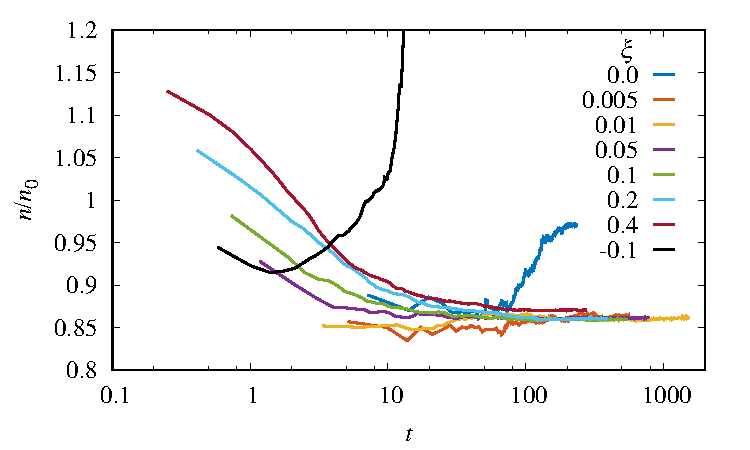
\includegraphics[width=0.55\textwidth]{./5applications-NREL/XiExploration.pdf}}
\end{figure}
%


%%%%%%%%
\subsubsection{1D fermions at finite temperature \label{sect:fermions_ft_1d}}
\paragraph{Repulsive interactions}

One of the first attempts to use CL for nonrelativistic fermions was Ref.~\cite{PRD95094502}, where the thermodynamics of a repulsive 1D Fermi gas
was calculated using that method as well third-order lattice perturbation theory (see \figref{DensityEoSCL1DFiniteT}). The density and pressure were
computed for a range of couplings and temperatures. The calculations were also compared with prior hybrid Monte Carlo results for attractive interactions,
where there is no sign problem and the convergence of the perturbative expansion could be assessed. On the repulsive side, CL was found to agree with
the third-order perturbative expansion at weak coupling and away from the virial region (where the fugacity is small), beyond which perturbation theory was expected
to break down.

That same work explored for the first time the use of a regulator to avoid uncontrolled excursions of the auxiliary field into the complex plane, as we explain next.
In those calculations, the excursions into the complex plane were highly problematic because the dependence of the action and the drift on the
auxiliary field $\sigma$ involved hyperbolic functions.  The HS transformation used in that work depends on $\sin \sigma$, and
the complexification $\sigma \to \sigma_R + i \sigma_I$ results in
%
\beq
\sin \sigma = \sin (\sigma_R) \cosh(\sigma_I) + i \cos (\sigma_R) \sinh(\sigma_I).
\eeq
%
As a consequence, a growing magnitude of $\sigma_I$ amounted to increasing the fermion-fermion coupling at an exponential rate. In such a situation, the calculation
would either stall or result in a converged but incorrect answer. This exponential growth is similar to the problem found in gauge theories,
as the complexified link variables representing the gauge field become unbounded in the same fashion in those theories.
For lattice calculations of gauge theories, Refs.~\cite{Lattice2016AttanasioJager,Lattice2017AttanasioJager} tackled the
problem of large excursions by so-called dynamic stabilization (see \secref{CLchallenges}). Following a similar idea, Ref.~\cite{PRD95094502} added a regulating term to the CL dynamics
controlled by a parameter $\xi$, such that the new CL equations became
%
\bea
\label{Eq:CLModifiedEqs}
\Delta \sigma_R &=& -\textrm{Re}\left[\frac{\delta S[\sigma]}{\delta \sigma}\right] \Delta t  - 2 \xi \sigma_R \Delta t + \eta \sqrt{\Delta t}, \\
\Delta \sigma_I &=& -\textrm{Im}\left[\frac{\delta S[\sigma]}{\delta \sigma}\right] \Delta t - 2 \xi \sigma_I \Delta t.
\eea
%
The new term in the action can be understood as a harmonic oscillator trapping potential, i.e. a restoring force that prevents the field from
running away. That modification introduces a systematic effect that needs to be studied for each quantity of interest as a function of $\xi$
as $\xi \to 0$. \figref{XiComparison} shows the running average of the density as a function of the Langevin time $t$ for several values of $\xi$
in the neighborhood of $0$. As is evident in that figure, there is a sizable window of small values of $\xi$
where CL converges.

%%%%%%%%%%%%%%%%%%

\paragraph{Spin-polarized systems}

Encouraged by the success of CL in calculating 1D systems with repulsive interactions, the follow-up study of Ref.~\cite{PhysRevD.98.054507}, extended the results of
Ref.~\cite{PRD95094502} to the spin-polarized case by introducing a non-vanishing asymmetry $\beta h = \beta (\mu_\uparrow - \mu_\downarrow)/2$.
Such an asymmetry leads to a sign problem for the case of attractive interactions and to a phase problem for repulsive interactions. As mentioned above, such a sign or
phase problem can be avoided in 1D using specific methods which, unfortunately, do not generalize to higher dimensions.
In the study of Ref.~\cite{PhysRevD.98.054507}, the density and magnetization equations of state were calculated and compared with perturbation theory,
imaginary polarization approaches, and the virial expansion. A sample of those results is reproduced in \figref{DensityLambda1}.

%%%%%%%%%%%%%%%%%%%%%%%%%%%%%%%%%%%%%%%%%
\subsection{Nonrelativistic fermions in three dimensions: the polarized unitary Fermi gas}
%
One of the most studied many-body systems in recent years is the so-called unitary Fermi gas (UFG). Due to a diverging s-wave scattering length, the microscopic information about the interaction between
the spin-up and -down particles is lost and all observed quantities can be written as universal functions of the fermion density and temperature (as these are the only scales left at our disposal). Its intricate
behavior is linked to various many-body phenomena, and moreover it is realized to an excellent precision in numerous cold atoms experiments, having led to a plethora of precise measurements of its unique
behavior.
%
\begin{figure*}[t]
	\centering
	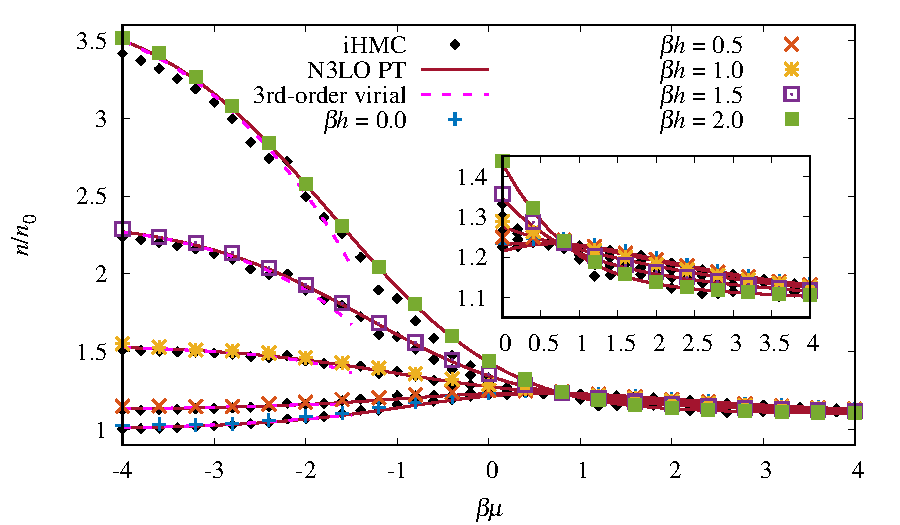
\includegraphics[width=0.49\columnwidth]{./5applications-NREL/Density_Attractive_L1.pdf}
	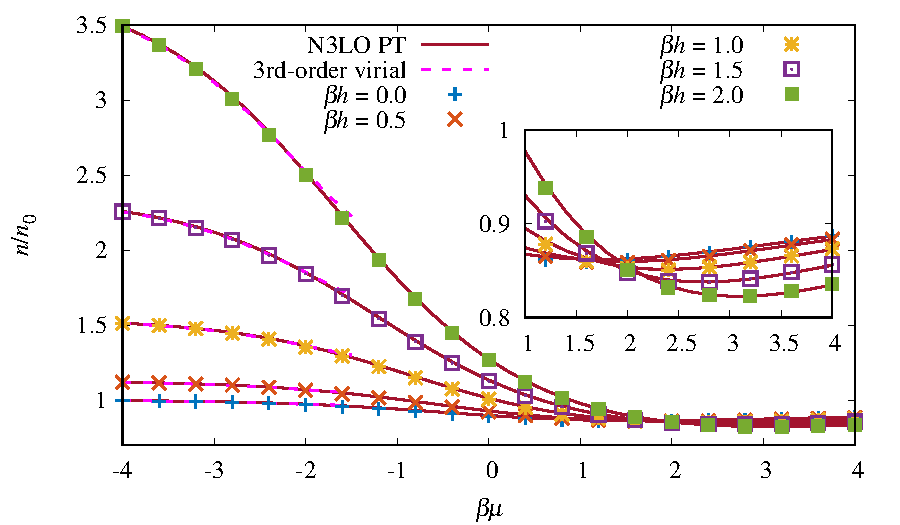
\includegraphics[width=0.49\columnwidth]{./5applications-NREL/Density_Repulsive_L1.pdf}
	\caption{\label{fig:DensityLambda1} Density equation of state $n = n_\uparrow + n_\downarrow$ normalized by the non-interacting, unpolarized counterpart $n_0$,
	{for attractive (left) and repulsive (right) interactions of strength $\lambda = \pm 1$.
	Insets: Zoom in on the region $\beta\mu > 0$ (left) and $\beta\mu > 1$ (right).}
	In all cases, the CL results are shown with colored symbols, iHMC results (from Ref.~\cite{PhysRevA.92.063609}) appear with
	black diamonds, perturbative results at third order are shown with solid lines, and virial expansion results
	appear as dashed lines.}
\end{figure*}
%

For SU(2) symmetric fermions, i.e. for equal numbers of spin-up and -down particles, it is possible -- albeit challenging -- to study the UFG with conventional Monte Carlo approaches. Past stochastic studies of
the UFG have been conducted using methods such as hybrid Monte Carlo (HMC) \cite{PhysRevA.85.051601, PhysRevLett.110.090401, PhysRevA.93.053604} and auxiliary field methods (AFQMC) on the
lattice \cite{Jensen2019, PhysRevA.84.061602, PhysRevB.73.115112} as well as various flavors of diagrammatic Monte Carlo methods \cite{PhysRevLett.121.130405, VanHoucke2012} in the continuum.

%Recent work expanded the application of CL to spin-polarized unitary fermions, which are by definition in 3D, where the sign problem cannot be circumvented via other methods.
%The equation of state of the unitary spin-polarized Fermi gas was determined and compared with the second-order virial expansion as well as experiment (for the unpolarized case).
%The results tracked closely with both the virial expansion and the experimental data, aside from some evidence of (controllable) finite-size effects~\cite{2018UFGviaCL}.

By introducing a finite chemical potential asymmetry the SU(2) symmetry is broken, creating a sign problem. To address that issue, the CL method was applied to the spin-polarized unitary Fermi gas for the first time in Ref.~\cite{2018UFGviaCL}, finding excellent agreement with available benchmark results. In the left panel of \figref{ufg_eos}, the density equation of state is shown for a balanced gas in comparison to previously obtained results from DHMC \cite{PhysRevA.85.051601} and bold diagrammatic Monte Carlo (BDMC) \cite{VanHoucke2012} studies, as well as experimental values from the MIT group \cite{VanHoucke2012}. Across a wide range of $\beta\mu$ values, excellent agreement was reported down to low temperatures.
In the vicinity of the phase transition to superfluidity, however, the CL results, along with all other theoretical values, start to deviate from the experimental values, which is attributed to finite lattice effects and can, in principle, be mitigated by extending the box sizes beyond $N_x = 11$.
%
\begin{figure}[t]
  \centering
  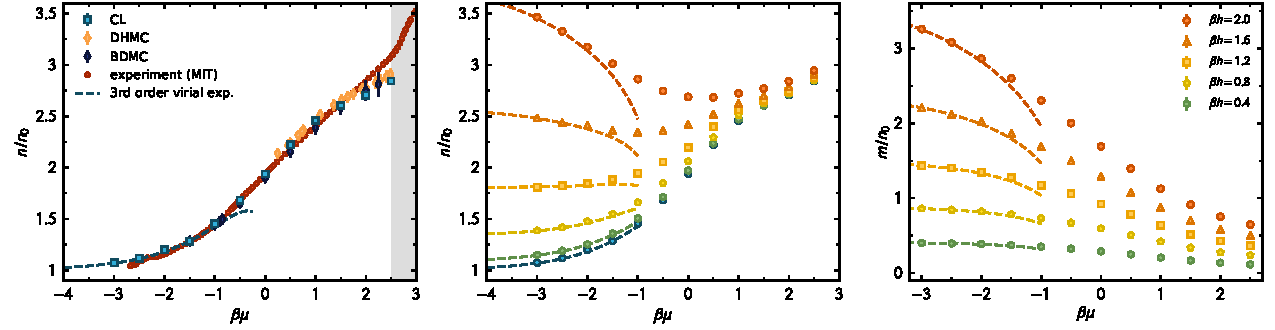
\includegraphics[width=\columnwidth]{./5applications-NREL/ufg_eos.pdf}
  \caption{\label{fig:ufg_eos} (Left) Density in units of the non-interacting density as a function of the dimensionless parameter $\beta \mu$ for the balanced Fermi gas. Additionally, comparison to theoretical values (BDMC \cite{VanHoucke2012}, DHMC \cite{PhysRevA.85.051601}) and experimental values from the MIT group \cite{VanHoucke2012} are shown. (Center) Density in units of the non-interacting density as a function of $\beta \mu$ for the polarized Fermi gas, compared to the third order virial expansion at high temperatures. (Right) Magnetization in units of the non-interacting density as a function of $\beta \mu$ compared to the 3rd order virial expansion at high temperatures.}
\end{figure}
%

In the central and right panels of \figref{ufg_eos} the density and magnetic EOS are shown, respectively. It is important to note here that these system can be dealt with by essentially the same computational effort as in the spin-balanced case, whereas a re-weighting approach would suffer from an exponential increase in computational effort. As can be appreciated from the figure, excellent agreement with the virial expansion (see e.g. \cite{LIU201337}) is achieved at high temperatures, which gives confidence on the reliability of the CL results in that regime. Moving towards lower temperatures, the virial expansion is expected to break down, whereas the CL results continue to evolve smoothly across the entire parameter range studied.

%
While the virial expansion allows for a validation of CL results at high temperatures, no benchmark is available in the literature at finite spin polarization. As a way to perform an internal consistency check, Ref.~\cite{2018UFGviaCL} exploited one of the Maxwell relations known from statistical mechanics. More specifically, the equality in cross derivatives of $\mathcal Z$ with respect to $\beta h$ and $\beta \mu$, i.e.
%
\beq
\left( \frac{\partial n}{\partial (\beta h)} \right)_{\beta\mu} = \left( \frac{\partial m}{\partial (\beta \mu)} \right)_{\beta h},
\eeq
%
should be satisfied for all parameter values. The two different derivatives are shown as red and blue symbols in \figref{ufg_maxwell}. While the agreement was suggested already in the EOS for the virial regime, the excellent agreement across almost all values of $\beta\mu$ and $\beta h$ is a non-trivial verification and provides another argument for the validity of the CL calculation. We emphasize that these data points were obtained by completely independent calculations, i.e. no prior information entered this cross check.
%
\begin{figure}
  \centering
  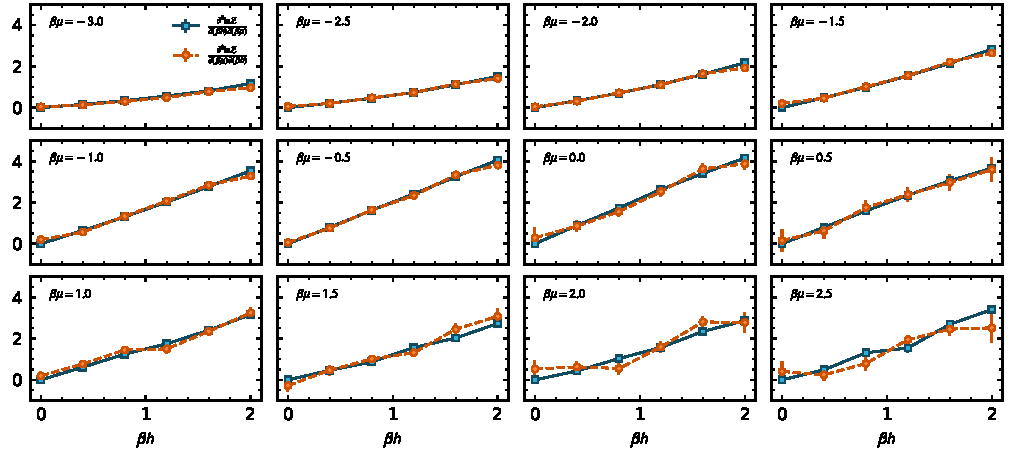
\includegraphics[width=\columnwidth]{./5applications-NREL/ufg_maxwell.pdf}
  \caption{\label{fig:ufg_maxwell} Second derivatives of $\ln\mathcal{Z}$ to verify Maxwell relations as a function of $\beta h$. Every plot corresponds to a fixed value of $\beta\mu$. The lines are guides to the eye.}
\end{figure}


%more? "To characterize the universal thermodynamics of the polarized UFG, we computed the density $n$, magnetization $m$, and normalized magnetic susceptibility $\Xi_{M}$ [...] as functions of the dimensionless chemical potential $\beta_{\mu}$ [...] dimensionless chemical potential difference $\beta_{h}$."
%"We carried out a nonperturbative characterization of the density and magnetization EOS of the UFG at finite temperature. To that end, we implemented a finite-temperature stochastic lattice approach that addresses the sign problem by going to the complex plane, i.e. we used the complex Langevin approach and presented our results as a function of $\beta \mu$ and $\beta h$. We emphasize that those results represent testable predictions for universal properties of quantum manybody physics in the unitary limit, as realized in particular with ultracold gases. In the unpolarized case, we recover state-of-the-art results. At finite polarization, our answers agree with the third-order virial expansion for $\beta \mu ~2.0$, where the expansion is expected to be valid. As in our 1D studies [16], however, the expansion deteriorates as $\beta h$ is increased. "


\end{document}
